\documentclass[preview=true, tikz=true]{standalone}

\usetikzlibrary{shapes.geometric, arrows,quotes, positioning}

\begin{document}
    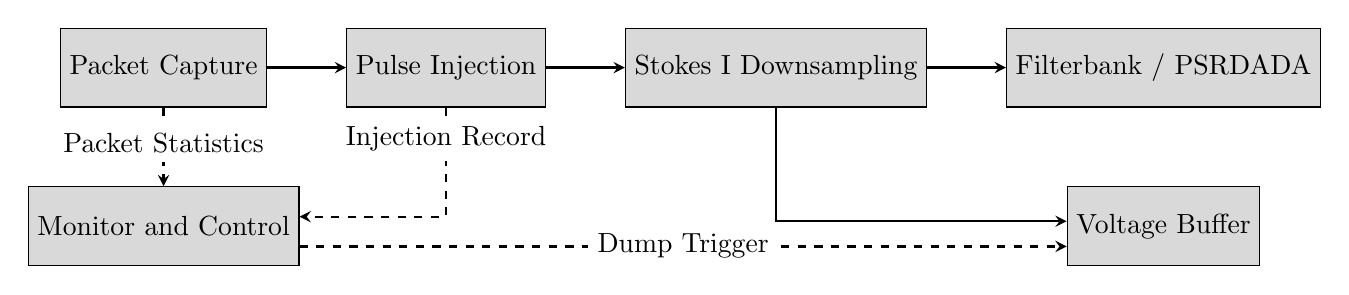
\begin{tikzpicture}
        \node[draw,minimum width=1cm,minimum height=1cm,align=center,fill=gray!30] (cap) at (0,0) {Packet Capture};
        \node[draw,minimum width=1cm,minimum height=1cm,align=center,fill=gray!30] (inject) [right = of cap] {Pulse Injection};
        \node[draw,minimum width=1cm,minimum height=1cm,align=center,fill=gray!30] (downsample) [right = of inject] {Stokes I Downsampling};
        \node[draw,minimum width=1cm,minimum height=1cm,align=center,fill=gray!30] (exfil) [right = of downsample] {Filterbank / PSRDADA};
    
        \node[draw,minimum width=1cm,minimum height=1cm,align=center,fill=gray!30] (buffer) [below = of exfil] {Voltage Buffer};
        \node[draw,minimum width=1cm,minimum height=1cm,align=center,fill=gray!30] (mnc) [below = of cap] {Monitor and Control};
    
        \draw[-stealth, thick] (cap) --  (inject);
        \draw[-stealth, thick] (inject) --  (downsample);
        \draw[-stealth, thick] (downsample) --  (exfil);
        \draw[-stealth, thick] (downsample) |-  ([yshift=0.25cm]buffer);
        \draw[-stealth, thick, dashed] (cap) -- node[anchor=mid, fill=white] {Packet Statistics}  (mnc);
        \draw[-stealth, thick, dashed] (inject) |- node[anchor=south,fill=white,yshift=0.70cm] {Injection Record} ([yshift=0.25cm]mnc);
        \draw[-stealth, thick, dashed] ([yshift=0.25cm]mnc.south east)  -- node[anchor=mid, fill=white] {Dump Trigger} ([yshift=0.25cm]buffer.south west);
    \end{tikzpicture}
\end{document}
